\documentclass[10pt]{article}
\usepackage{algorithm,algorithmic,amsmath,amsthm,mathtools,commath,xcolor,graphicx}
\graphicspath{ {./} }
\title{TDA251\\Solutions for Assignment 1}
\author{Wang QuFei\\900212-6952\\qufei@student.chalmers.se}

\begin{document}
\maketitle
\section*{Excrcise 1}
Given a graph $G = (V,E)$, let $X$ be an arbitray set of nodes returned by the greedy solution, Y be an independent set with maximum size of nodes. We prove that
										 \[\abs{X} \geq \abs{Y}/\Delta\]
Denote $X := \{x_{1}, x_{2},\ldots, x_{m}\}$, where $x_{i}$ are the nodes selected by the greedy algorithm in sequence. Correspondingly, denote $A_{i} \subseteq V$ as the set of nodes consists of $x_{i}$ and the nodes removed together as its neighbours in iteration.\\
Consider $B_{i} \coloneqq A_{i} \cap Y$, we claim that $B_{i}$ can not be empty. This is because at least $B_{i}$ could contain $x_{i}$ as its element, for by rule of our greedy algorithm, there is no edge between $x_{i}$ and any other nodes in $V \setminus A_{i}$, which means if $B_{i}$ does not contain any other elements different from $x_{i}$ in $A_{i}$, it must contain $x_{i}$.\\
Observe that, in the worst case, $B_{i}$ has only one element $x_{i}$, because $x_{i}$ has an edge with all of its neighbours. In the best case, $B_{i}$ has potentially all the neighbours of $x_{i}$, supposing there's no edge between any two of these nodes. Thus we have the following inequation
								\[1 \leq \abs{B_i} \leq \Delta\]
Thus we have
								\[\frac{1}{\Delta} \leq \frac{\abs{\{x_i\}}}{\abs{B_{i}}} \leq 1\]
Notice that 
								\[Y = B_{1} \cup B_{2} \cup \ldots \cup B_{m}\]
and
								\[B_{i} \cap B_{j} = \emptyset, i \neq j \]
Finally we have 
								\[\left( \abs{X} = \sum_{i=1}^{m}\abs{\{x_{i}\}} \right) \geq \left( \sum_{i=1}^{m}\frac{\abs{B_{i}}}{\Delta} = \frac{\abs{Y}}{\Delta} \right)\]
\qed
\section*{Excrcise 2}
A greedy algorithm can be given as follows:
\begin{algorithm}
\begin{algorithmic}
\STATE Let $S$ be the site of n sites, $S'$ be the set of remaining sites need to be covered and $C$ be the set of centers.\\
\STATE Initialize $S' = S$, $C = \emptyset$
\WHILE{$S' \neq \emptyset$}
\STATE{
Select any site $s \in S'$ and add $s$ in $C$\\
Delete $s$ and all the sites within Manhattan distance $r$ from $s$ from $S'$}
\ENDWHILE
\RETURN C
\end{algorithmic}
\end{algorithm}

We claim that:
\begin{enumerate}
	\item The algorithm can run in $O(n^2)$ time
	\item Every site has a distance at most $r$ from some center
	\item The center set returned has at most $4k$ elements
\end{enumerate}
$(1)$ is true for in the worst case when any two sites have distance larger than $r$, we have to compare the distance between the selected site $s$ and all the remaining sites in $S'$ with $r$.\\
$(2)$ is guaranteed by the way of the deletion of sites that within distance $r$ of the newly selected center site.\\
$(3)$ is also true for the geometric nature of Manhattan distance. Suppose $C^*$ is the optimal solution that has $k$ centers selected. During the execution of our algorithm, for any newly selected center $c = (x, y)$ there must be a center $c' \in C^*$ that covers it within $r$ distance. Supporse $c'$ has coordinate $(x', y')$. Observe that the area covered by $c'$ is the square identified by these four points $p_w = (x' - r, y')$, $p_n = (x', y' + r)$, $p_e = (x' + r, y')$, $p_s = (x', y' - r)$. Denote this area as $A_{c'}$, which is depicted in the image below.\\
\begin{figure}[h]
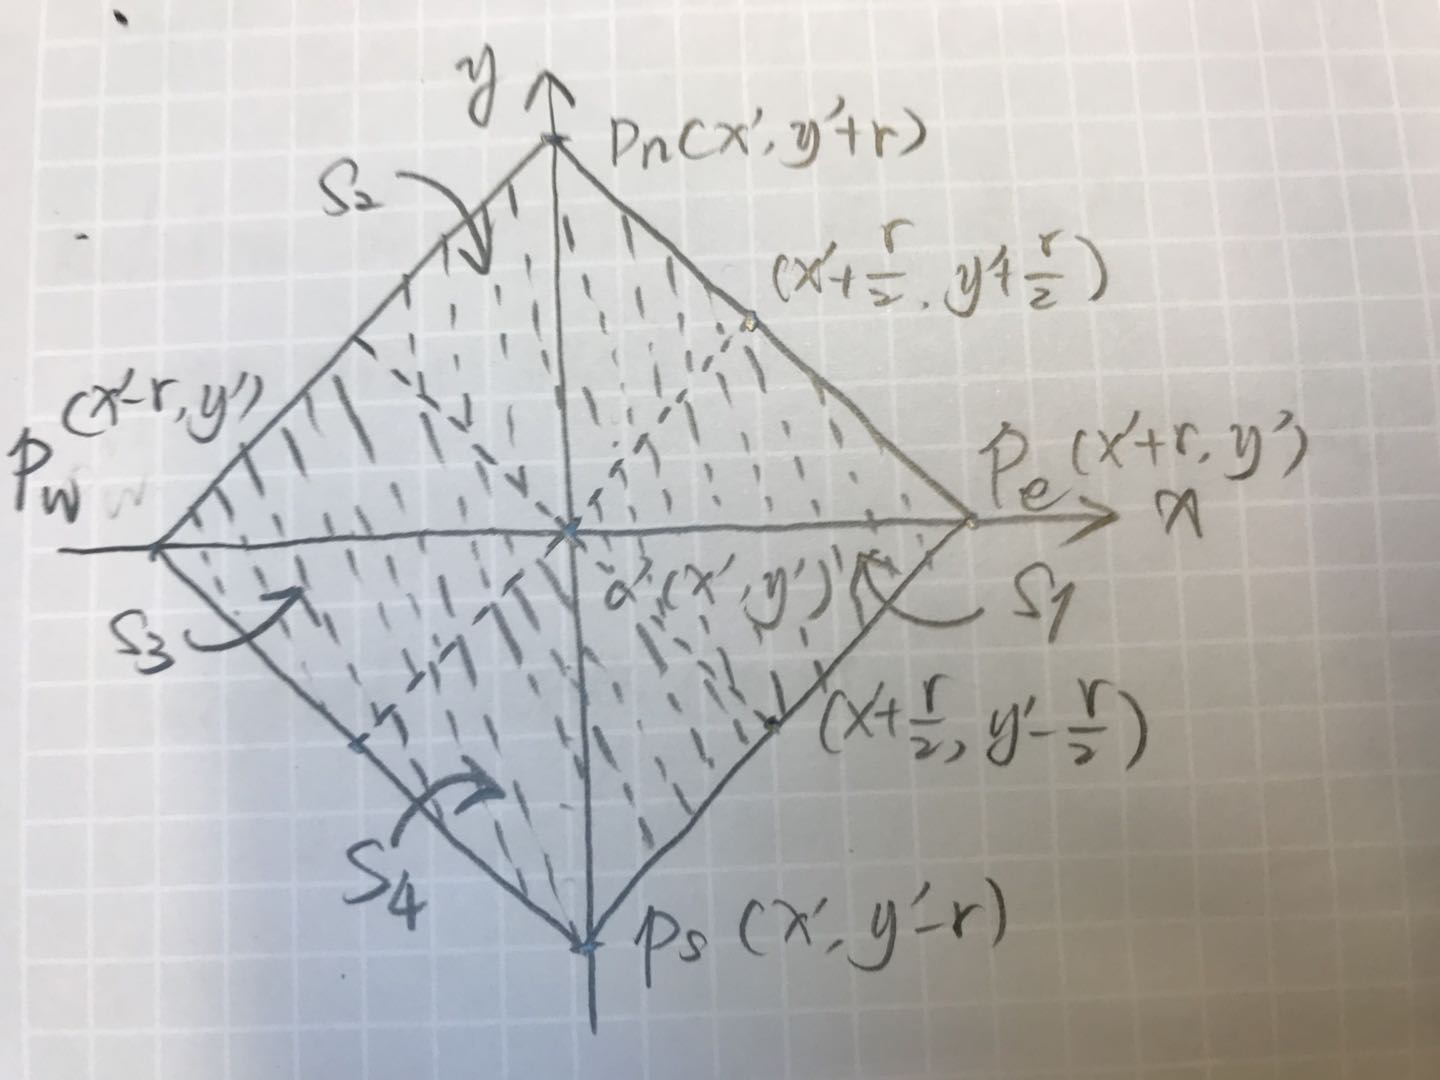
\includegraphics[width=10cm, height=9cm]{area}
\end{figure}
\begin{itemize}
	\item If $c = c'$. Then for the current while-loop, the greedy algorithm does not produce more centers than $C^*$.
	{\color{red}
	\item If $c$ falls into the inner square $S_1$ denoted by $(x',y')$,$(x'+ \dfrac{r}{2}, y' + \dfrac{r}{2})$,$(x' + r, y')$,$(x' + \dfrac{r}{2}, y' - \dfrac{r}{2})$. Observe that any two points in this area have Manhattan distance no more than $r$, which means all sites in this area covered by $c'$ are also covered by $c$.
	\item Similarly, if $c$ falls into $S_2$(denoted by $(x',y')$, $(x' - \dfrac{r}{2}, y' + \dfrac{r}{2})$, $(x', y' + r)$, $(x'+ \dfrac{r}{2}, y' + \dfrac{r}{2})$), or $S_3$(denoted by $(x',y')$, $(x' - \dfrac{r}{2}, y' - \dfrac{r}{2})$, $(x' - r, y')$, $(x'- \dfrac{r}{2}, y' + \dfrac{r}{2})$), or $S_4$(denoted by $(x',y')$, $(x' + \dfrac{r}{2}, y' - \dfrac{r}{2})$, $(x', y' - r)$, $(x'- \dfrac{r}{2}, y' - \dfrac{r}{2})$), all the sites in that particular area covered by $c'$ would also be covered by $c$. Thus, during the course of our greedy algorithm, at most $4$ sites need to be choosen to cover all the sites originally covered by some center $c' \in C^*$. 
	}
\end{itemize}
It follows that the output of our greedy algorithm has at most $4k$ elements.\qed
\end{document}